\let\cleardoublepage\clearpage
\appendix
	\crefalias{section}{appchap}
	\let\cleardoublepage\clearpage
	\chapter{Sujet du stage}
	\let\cleardoublepage\clearpage
	\label{apx.SujetStage}
	\section*{Répartition du séquenceur multimedia i-score sur plusieurs machines}
	
	Le projet ANR Open Scenario System for Interactive Application (OSSIA)
	souhaite offrir aux développeurs des outils génériques pour l'écriture
	et l'exécution de scenarios ouverts et multi-utilisateurs pour le
	spectacle vivant pilotant des processus multimedia.
	
	Le logiciel i-score a été développé dans le cadre de la plateforme de
	recherche Virage, financée par l'ANR. Ce logiciel permet de concevoir
	des scenarios multimedias, mêlant son, lumière et vidéo, et de moduler
	leur exécution en temps-réel pour s'adapter au temps du plateau dans
	le cadre du spectacle vivant. Le système comprend deux parties :
	
	- un éditeur permettant de composer un scenario avec la notion
	d'objets temporels statiques ou interactifs reliés par des relations
	temporelles sur une time-line.
	
	- un moteur d'exécution opérant sur une représentation du scenario
	sous forme de réseau de petri.
	
	Dans le cadre de ce stage, il s'agit de répartir le réseau de Petri
	sur plusieurs machines afin de le rendre multi-utilisateur. Ainsi, les
	régisseurs son, lumière, vidéo etc. pourraient interagir chacun avec
	la partie qui concerne son média. Il faudra donc concevoir une
	architecture répartie et s'interesser particulièrement aux
	synchronisations compte tenu des délais de communication et des
	horloges multiples.
	
	Le stagiaire intégrera une équipe de 3 ingénieurs du LaBRI et du
	SCRIME et de 5 chercheurs permanents du LaBRI.
	\let\cleardoublepage\clearpage
	\chapter{Exemple OSSIA}
	\let\cleardoublepage\clearpage
	\label{apx.OSSIAExemple}
	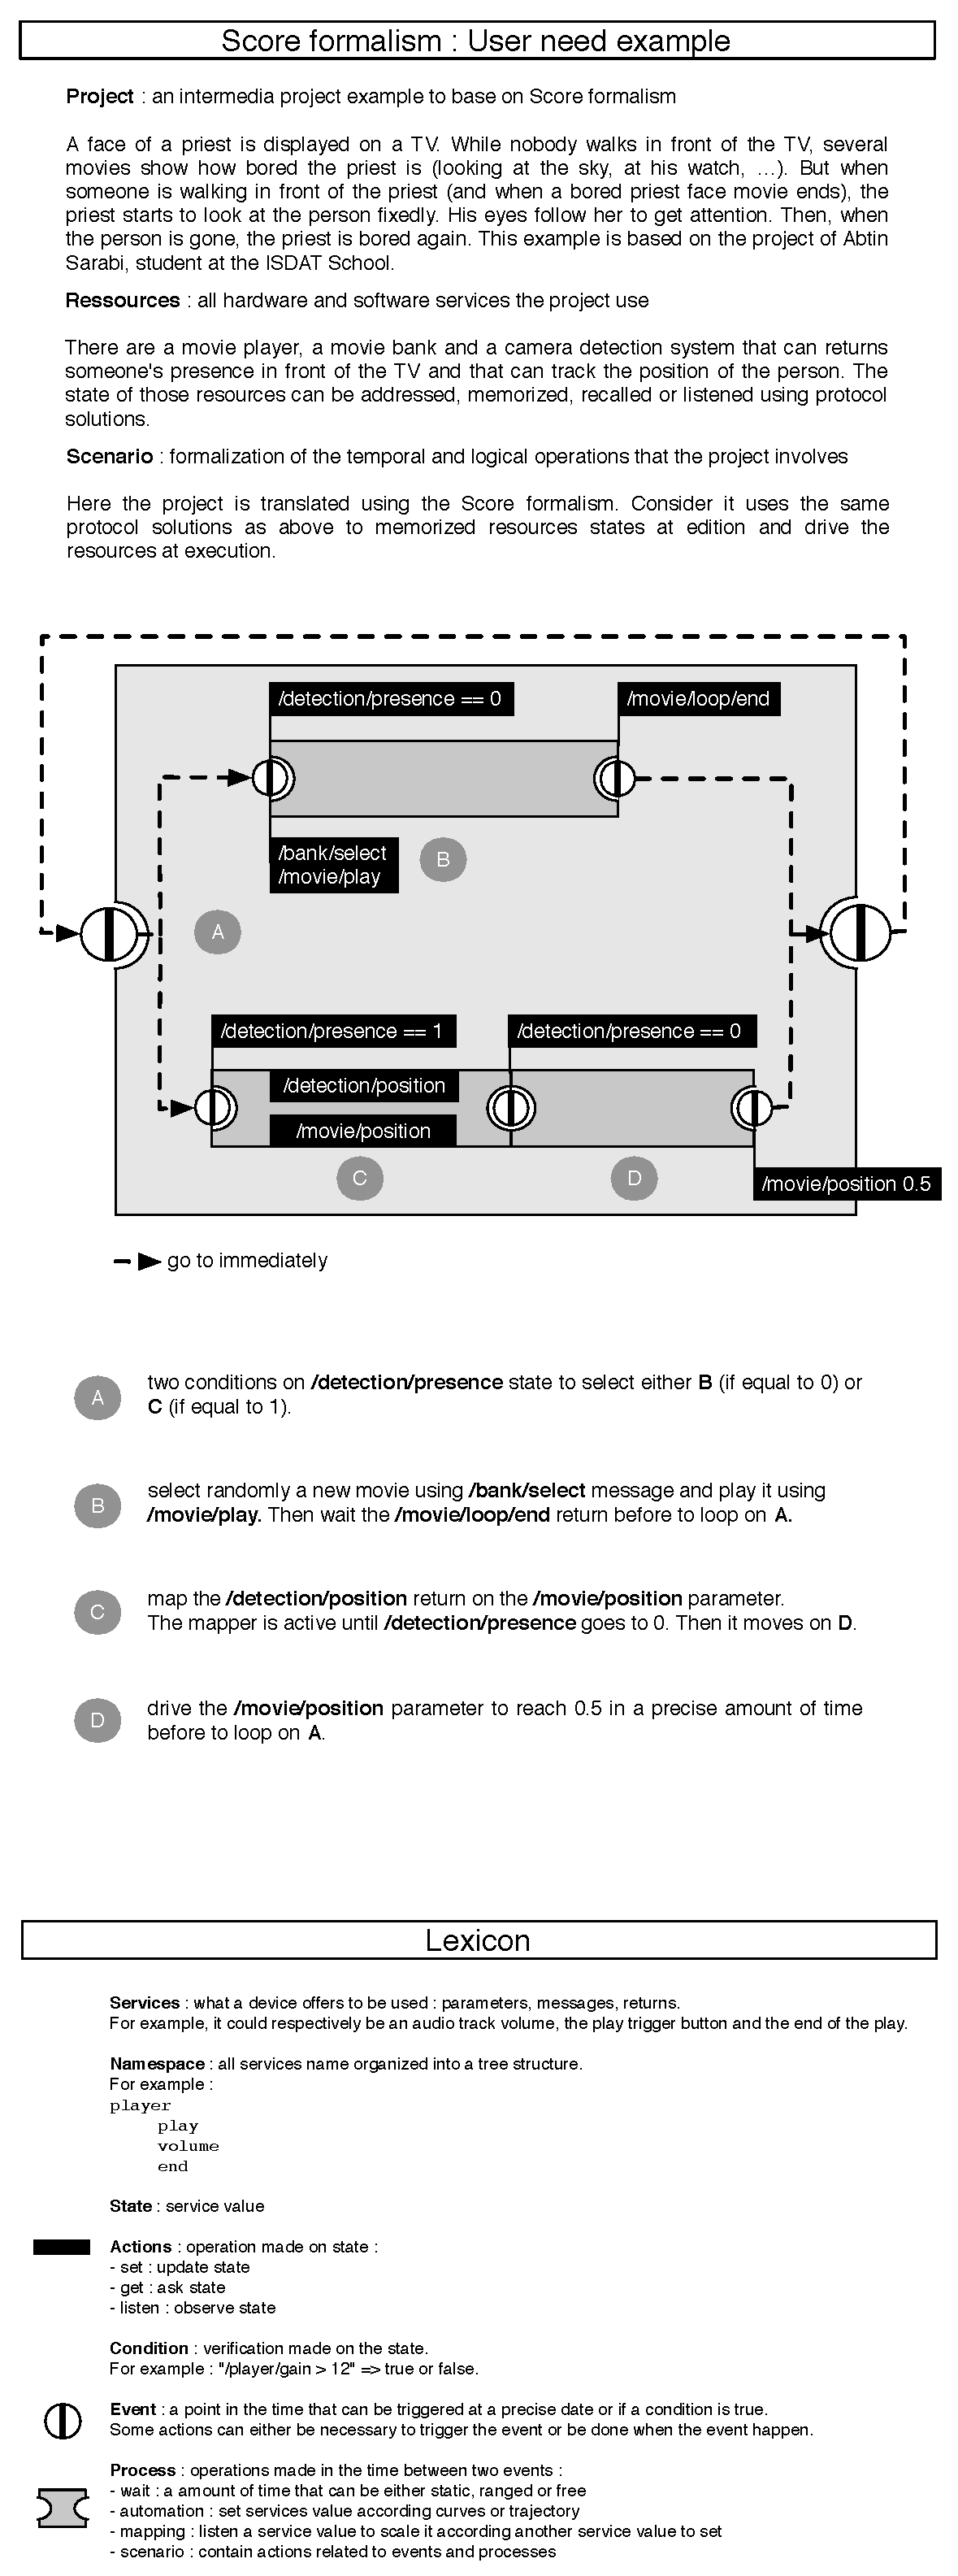
\includegraphics[clip,trim=0cm 28cm 0cm 0cm, width=1.00\textwidth]{images/moineOSSIA.pdf}
	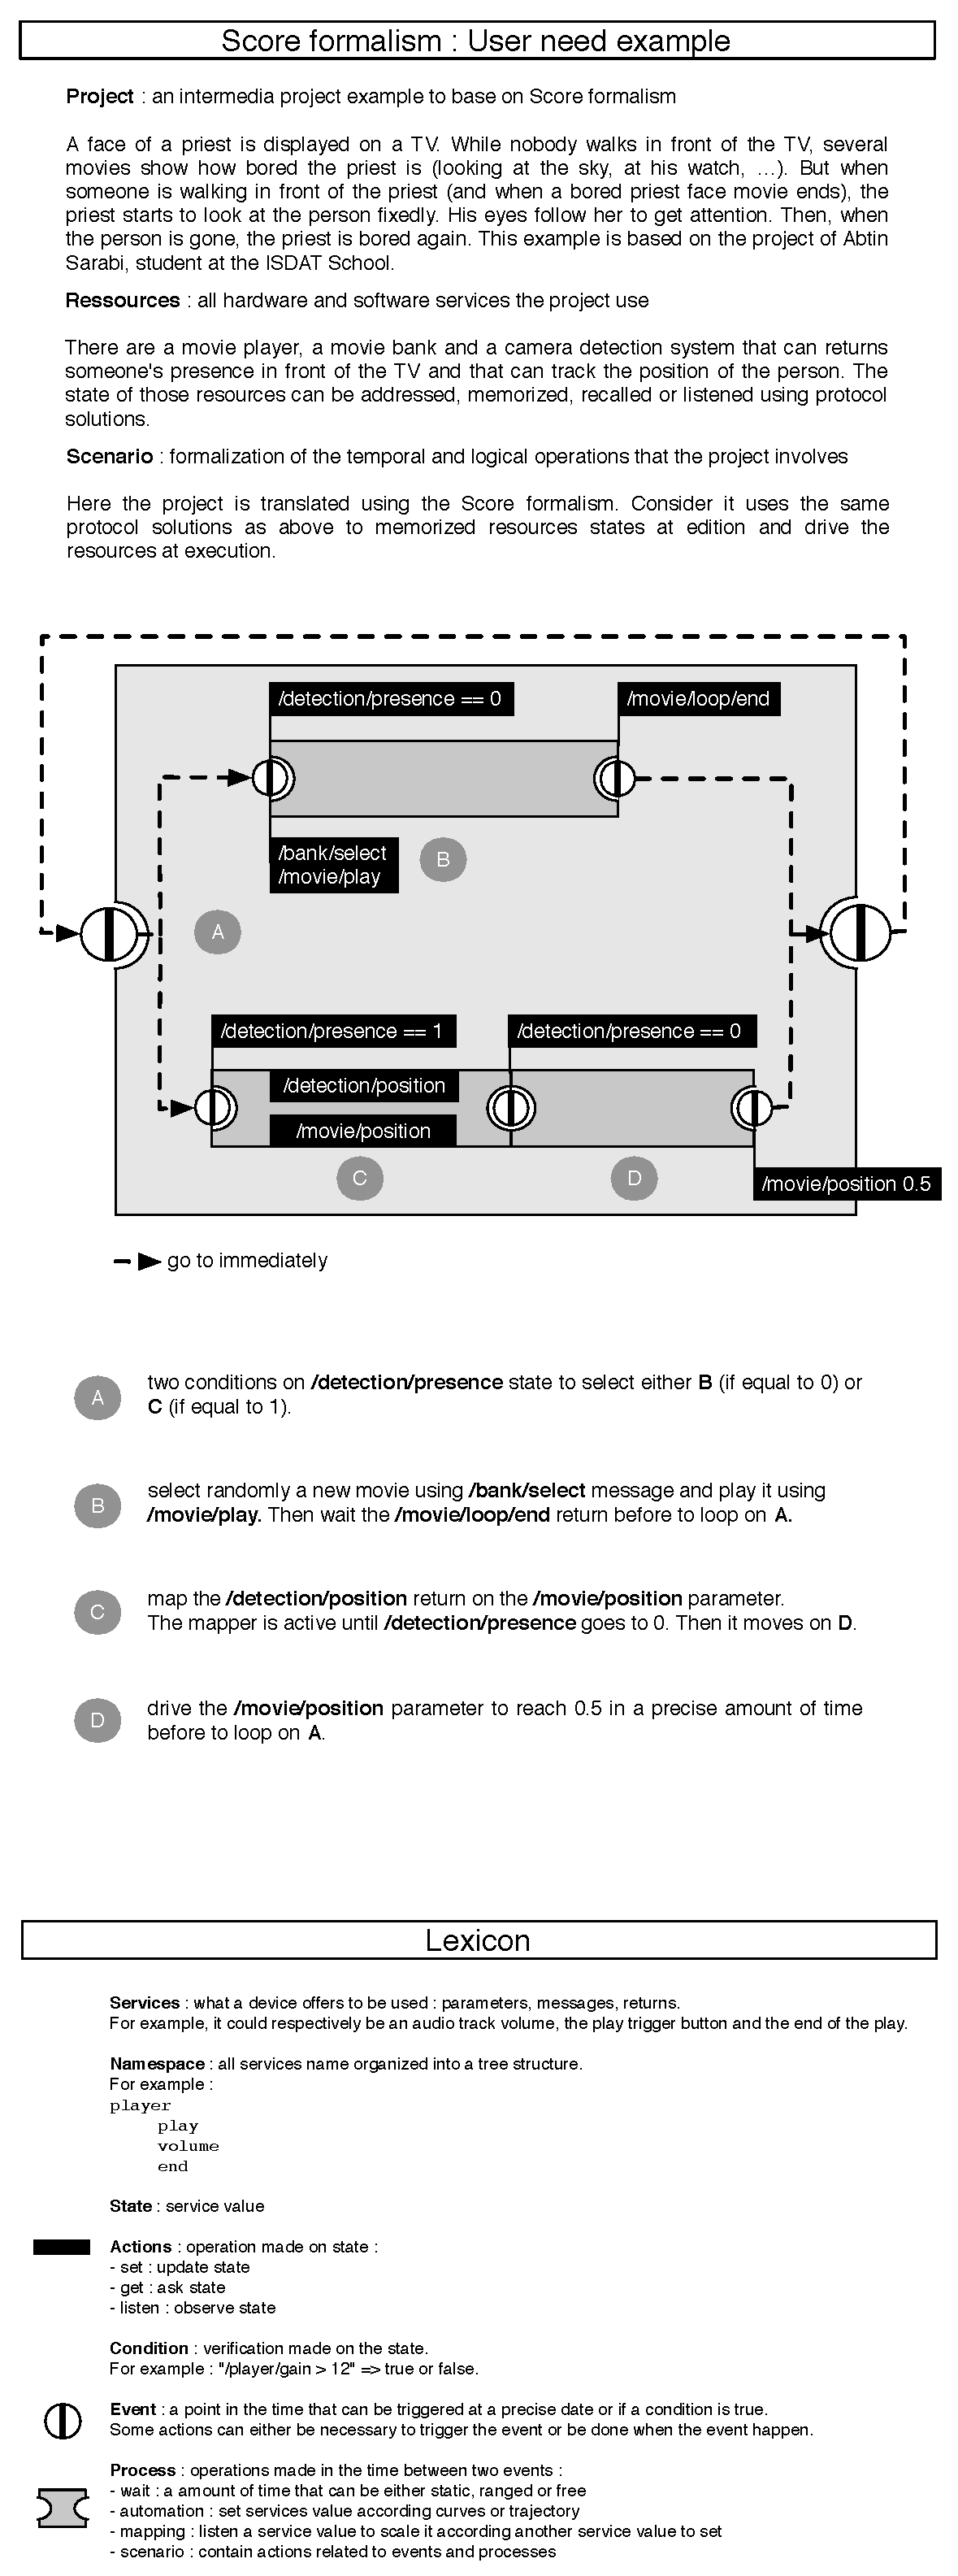
\includegraphics[clip,trim=0cm 0cm 0cm 26cm, width=1.00\textwidth]{images/moineOSSIA.pdf}